\documentclass[9pt,t]{beamer}

%-------------------------------------------------
%   THEMES & PACKAGES
%-------------------------------------------------
\usetheme[progressbar=frametitle]{metropolis}
\usepackage[belowskip=-15pt]{caption}
\usepackage{graphicx}
\usepackage{subcaption}
\usepackage{wrapfig}

%-------------------------------------------------
%   Settings
%-------------------------------------------------
\graphicspath{{../images/}{../../images/}}
\setbeamertemplate{footline}[text line]{%
    \parbox{\linewidth}{\vspace*{-8pt}\insertshorttitle\hfill\insertshortsubtitle\hfill\insertshortauthor\hfill\insertpagenumber}}
\setbeamertemplate{navigation symbols}{}

%-------------------------------------------------
%   TITLE
%-------------------------------------------------
\title{Neural Networks}
\subtitle{Final Review}
\date{\today}
\author{Minh Nguyen}
\titlegraphic{\hfill
\includegraphics[height=0.7cm]{h-brs-logo.png}}

%-------------------------------------------------
%   COMMANDS
%-------------------------------------------------
\newcommand{\picEqHereWidth}[2] { %
    \begin{figure}[htp] 
        \centering
        \includegraphics[width=#2]{#1}
    \end{figure}
}
\newcommand{\picHereWidth}[4] { %
    \begin{figure}[htp] %
        \centering
        \includegraphics[width=#4]{#1} %
        \caption{#2} %
        \label{#3}
    \end{figure} %
}
%-------------------------------------------------
%   BEGIN
%-------------------------------------------------
\begin{document}

%-------------------------------------------------
\maketitle

%-------------------------------------------------
\begin{frame}{Artificial Neural Networks}
    \begin{alertblock}{ANN definition}
        \begin{itemize}
            \item massively parallel distributed processor
            \item (made up of) simple processing units
            \item (good at) storing experiential knowledge \& making it available for use
            \item resembles the brain
        \end{itemize}
    \end{alertblock}
    \begin{alertblock}{Neuron definition}
        A neuron is a \textbf{basic info processing unit of a NN}, consisting of:
        \begin{itemize}
            \item set of connecting links (\textbf{weights} or synapses)
            \item an \textbf{adder} function (linear combiner): computes weighted inputs
            \item \textbf{activation function} (squashing function): limits neuron output. Types:
            \begin{itemize}
                \item threshold (McCulloch-Pitts model): step function
                \item piece-wise linear: linear on $(\frac{-1}{2}, \frac{1}{2})$, like step function elsewhere.
                \item sigmoid.
            \end{itemize}
        \end{itemize}
    \end{alertblock}
\end{frame}

%-------------------------------------------------
\begin{frame}{Artificial Neural Networks}
    \picHereWidth{neuron_graph}{Neuron graph}{fig:neuron}{0.7\linewidth}
    \begin{alertblock}{Types of NN architectures}
        \begin{itemize}
            \item single layer feed forward (neurons organized)
            \item multilayer feed forward (acyclic layers)
            \item recurrent (acyclic layers)
        \end{itemize}
    \end{alertblock}
\end{frame}

%-------------------------------------------------
\begin{frame}{Artificial Neural Networks}
    \begin{figure}[htp!]
        \centering
        \begin{subfigure}{.5\textwidth}
            \centering
            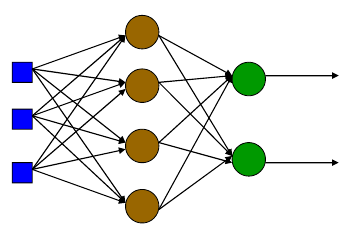
\includegraphics[width=.7\linewidth]{mlp.png}
        \end{subfigure}%
        \begin{subfigure}{.5\textwidth}
            \centering
            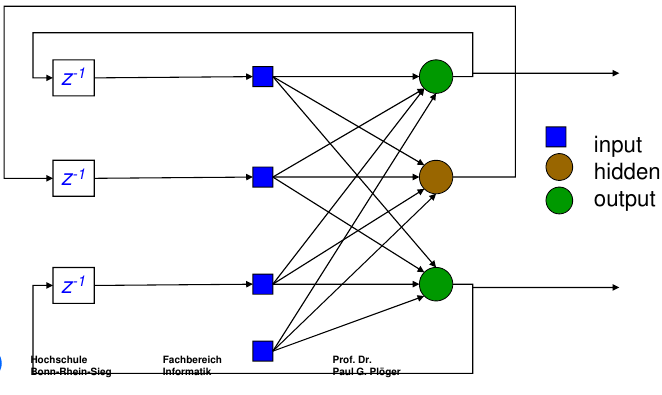
\includegraphics[width=\linewidth]{rnn.png}
        \end{subfigure}
        \caption{MLP and RNN networks}
    \end{figure}
    \begin{alertblock}{Knowledge rules in ANNs}
        \begin{itemize}
            \item similar inputs from similar classes produce similar representations
            \item items from separated classes should receive different representations
            \item important features should be represented using large number of neurons
            \item prior info and \textbf{invariance} should be built-in to the network
            \begin{itemize}
                \item invariance by structure: $w_{ij} = w_{ji}$
                \item invariance by training: many examples
                \item invariant feature space
            \end{itemize}
        \end{itemize}
    \end{alertblock}
\end{frame}

%-------------------------------------------------
\begin{frame}{Artificial Neural Networks}
    \picHereWidth{reinforce_learn.png}{Reinforcement learning}{fig:rf}{0.5\linewidth}
    \begin{alertblock}{Learning paradigms}
        \begin{itemize}
            \item supervised: build input-output relation known through examples
            \item unsupervised: model properties of inputs
            \item reinforcement learning: learn from outputs -- whether the output is good or bad.
        \end{itemize}
    \end{alertblock}
\end{frame}

%-------------------------------------------------
\begin{frame}{Artificial Neural Networks}
    \begin{alertblock}{Classification vs regression}
        \begin{itemize}
            \item regression outputs continuous values, whereas classification outputs discrete class labels
            \item regression examples: system identification, inverse modeling, controller
            \item classification examples: pattern matching,.
        \end{itemize}
    \end{alertblock}
    \begin{alertblock}{Similarity between polynomial curve fitting and NN regression}
        \begin{itemize}
            \item Similar formulation: polynoms $y = \sum_{j = 0}^{M} w_j x_j$; NN $y = f (\textbf{w}, \textbf{x})$
            \item Same error criterion $E = \sum_{p = 1}^{P}(y^p - t^p) ^2$
            \item Min error solution: polynoms -- quadratic in $\textbf{w}$, min(E) is solution of a set of linear equations; NN -- nonlinear in $\textbf{w}$, solve for local minima
        \end{itemize}
    \end{alertblock}
    \begin{alertblock}{Learning vs. generalization}
        \begin{itemize}
            \item Learning: find parameters $\textbf{w}$ to minimize error $ E $ given a set of examples
            \item Generalization: assign output value $ y $ to a new input $ x $ given $ \textbf{w} $
        \end{itemize}
    \end{alertblock}
\end{frame}

%-------------------------------------------------
\begin{frame}{Artificial Neural Networks}
    \begin{alertblock}{Overfitting}
        NN are \textbf{universal approximation models} with (relatively) \textbf{low complexity} $ \Rightarrow $ prone to overfitting
    \end{alertblock}
    \begin{alertblock}{model complexity}
        \begin{itemize}
            \item hard to compromise between performance and complexity $ \Rightarrow  $ control \emph{effective} complexity, use new error $ \tilde{E} = E + \lambda \Omega $ with penalty term:
            \[ \Omega = \frac{1}{2} \int \left(\frac{d^2 y}{x^2}\right)^2 dx \]
            \item many possible forms of $ \Omega $ and $ \lambda $ is hard to adjust.
        \end{itemize}
    \end{alertblock}
    \begin{alertblock}{Curse of dimensionality}
        \begin{itemize}
            \item More features lead to worse performance
            \item For few data samples dimension should be low
        \end{itemize}
    \end{alertblock}
\end{frame}

%-------------------------------------------------
\begin{frame}{Single layer learning}
    \picHereWidth{learning.png}{Learning process}{fig:learning}{0.6\linewidth}
    \begin{alertblock}{Perceptron learning for classification}
        \begin{figure}[htp!]
            \centering
            \begin{subfigure}{.3\textwidth}
                \centering
                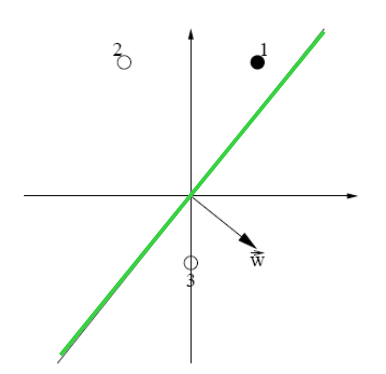
\includegraphics[width=\linewidth]{perceptron_learning1.png}
            \end{subfigure}%
            \begin{subfigure}{.3\textwidth}
                \centering
                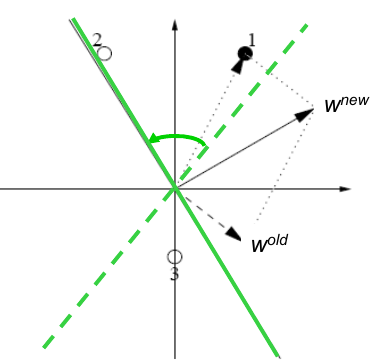
\includegraphics[width=\linewidth]{perceptron_learning2.png}
            \end{subfigure}
            \begin{subfigure}{.3\textwidth}
                \centering
                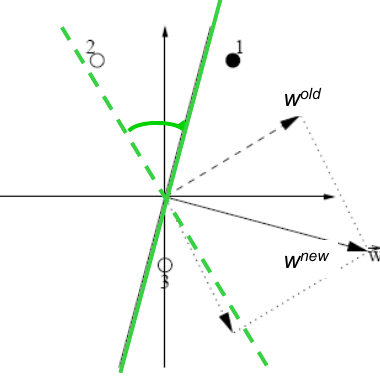
\includegraphics[width=\linewidth]{perceptron_learning3.png}
            \end{subfigure}
        \end{figure}
        \picEqHereWidth{perceptron_learning_eq.png}{0.3\linewidth}
    \end{alertblock}
\end{frame}

%-------------------------------------------------
\begin{frame}{Single layer learning}
    \begin{alertblock}{Adaline learning for regression}
        Adaline (\textbf{Ada}ptive \textbf{Lin}ear \textbf{E}lement) architecture:
        \begin{itemize}
            \item perceptron with linear activation function
            \item learning: error correction derived from LMS:
            \[ w(n+1) = w(n) - \eta \nabla E(w(n)) \approx w(n) + \eta x(w e(n)) \]
        \end{itemize}
    \end{alertblock}
    \begin{alertblock}{Fixed-increment learning algorithm}
        \begin{enumerate}
            \item initialization: $ n = 1, (n) = 0 $
            \item activate perceptron by applying input $ x(n) $
            \item compute output: $ y(n) = step(w^T(n) x(n)) $
            \item adapt weight vector: if $ d(n) \neq y(n) $ $ \Rightarrow w(n+1) = w(n) + \eta e(n) x(n) $,
            where $ e(n) = +1 $ for $ \textbf{X}(n) \in C_1 $ and $ e(n) = -1 $ for $ \textbf{X}(n) \in C_2 $
            \item continuation: increment $n$ and go to activation (step 2)
        \end{enumerate}
    \end{alertblock}
\end{frame}

%-------------------------------------------------
\begin{frame}{Single layer learning}
    \begin{alertblock}{Convergence theorem}
        Proof that perceptron algorithm converges
        \begin{itemize}
            \item Let $ \mathbf{w_0} $ be such that $ \mathbf{w_0^T x}(n) > 0, ~ \forall \mathbf{x}(n) \in C_1 $
            \item Let $ \alpha = \min(\mathbf{w_0^T x}(n)), ~ \forall \mathbf{x}(n) \in C_1 \Rightarrow $ Cauchy-Schwarz inequality: $ ||\mathbf{w}(k+1)||^2 \geq \cfrac{k^2 \alpha^2}{||\textbf{w}_0||^2} $
            \item Let $ \beta  = \max(||\textbf{x}(n)||^2), ~ \forall \mathbf{x}(n) \in C_1  \Rightarrow ||\mathbf{w}(k+1)||^2 \leq k \beta $
            \item To satisfied both above conditions, perceptron algorithm must terminate in at most $ n_{max} $ iterations: $ n_{max} = \cfrac{\beta ||\textbf{w}_0||^2}{\alpha^2} $
        \end{itemize}
    \end{alertblock}
    \begin{alertblock}{Perceptron limitation}
        \begin{itemize}
            \item can only model linearly separable functions.
            \item can model AND, OR, COMPLEMENT but not XOR.
        \end{itemize}
    \end{alertblock}
\end{frame}

%-------------------------------------------------
\begin{frame}{Single layer learning}
    \begin{alertblock}{Adaline vs. Perceptron}
        \begin{itemize}
            \item Model: Adaline uses linear, perceptron uses nonlinear activation functions.
            \item Learning: Adaline's continuous, perceptron has finite number of iterations.
        \end{itemize}
    \end{alertblock}
    \begin{alertblock}{ANN learning definition}
        \begin{itemize}
            \item process by which \textbf{free parameters} of a NN \textbf{are adapted} in a desired way
            \item through a \textbf{process of stimulation} by the environment
            \item type of learning is determined by how the parameter update are performed.
        \end{itemize}
    \end{alertblock}
    \begin{alertblock}{1st learning rule -- Error Correction}
        \begin{itemize}
            \item Optimize cost function (instantaneous at time $ n $, local at output node $ k $): $ \mathcal{E}(n) = \frac{1}{2} e_k^2(n) $, where $ e_k(n) = d_k(n) - y_k(n) $
            \item Widrow-Hoff rule (delta rule) for weight update: $ w_{kj}(n+1) = w_{kj}(n) + \eta \Delta w_{kj}(n) = w_{kj}(n) + \eta e_k(n) x_j(n) $
        \end{itemize}
    \end{alertblock}
\end{frame}

%-------------------------------------------------
\begin{frame}{Single layer learning}
    \begin{wrapfigure}{r}{0.4\linewidth}
        \centering
        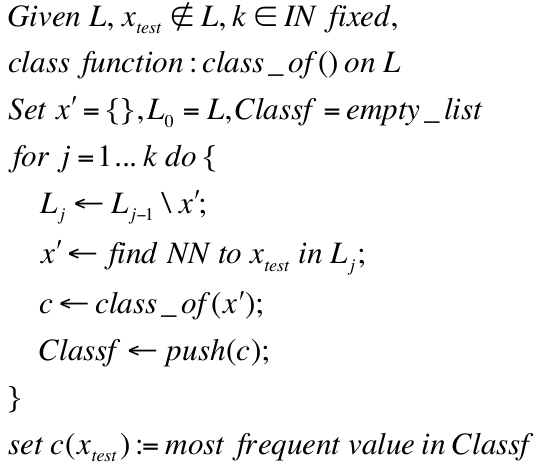
\includegraphics[width=\linewidth]{knn_algorithm.png} \\\hfill\\
        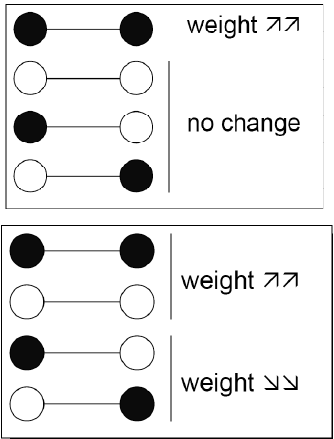
\includegraphics[width=0.8\linewidth]{hebbs.png}
    \end{wrapfigure}
    \begin{alertblock}{2nd learning rule -- Memory based}
        \begin{itemize}
            \item Nearest Neighbor definition: Given $ L = \{x_1, x_2,...,x_N\} $ and $ x_{test} \notin L $, $ x' \in L $ is nearest neighbor to $ x{test} \in L \iff \min_i d(x_i, x_{test}) = d(x', x_{test}) $
            \item k-NN algorithm (right).
        \end{itemize}
    \end{alertblock}
    \begin{alertblock}{3rd learning rule -- Hebbian}
        \begin{itemize}
            \item simultaneous~activation~of~2~neurons on either~side~of~a~synapse~$ \rightarrow $~synaptic weight increases
            \item asynchronous~activation~of~2~neurons~$ \rightarrow $~synaptic weight decreases
        \end{itemize}
    \end{alertblock}

\end{frame}

%-------------------------------------------------
\begin{frame}{Single layer learning}
    \begin{alertblock}{3rd learning rule -- Hebbian}
        \begin{itemize}
            \item 4 mechanisms: time-dependent, local, interactive, conjunctional/correlational.
            \item Covariance hypothesis: $ \Delta W_{kj}(n) = \eta (y_k - \bar{y})(x_j - \bar{x}) $
        \end{itemize}
    \end{alertblock}
    \begin{alertblock}{4th learning rule -- Competitive learning}
        \picEqHereWidth{competitive_learning}{0.7\linewidth}
    \end{alertblock}
\end{frame}

%-------------------------------------------------
\begin{frame}{Single layer learning}
    \begin{alertblock}{5th learning rule -- Boltzmann}
        \begin{itemize}
            \item Recurrent ANN with \textbf{binary neurons}.
            \item Operate by flipping -- probability of turning on:
            \picEqHereWidth{boltzmann_eq.png}{0.5\linewidth}
            \item Modes of operation: clamped and free running conditions:
            \picEqHereWidth{boltzmann_eq2.png}{0.4\linewidth}
            where $ \rho^+_{kj} $ and $ \rho^-_{kj} $ are correlation in clamped and free running states.
        \end{itemize}
    \end{alertblock}
\end{frame}

%-------------------------------------------------
\begin{frame}{Statistical Learning Theory}
    \begin{alertblock}{VC-Dimension}
        \begin{itemize}
            \item Given learning machine $ \mathbf{f} $ with vector of adjustable parameters $ \alpha $. Define probability of misclassification:
            \picEqHereWidth{prob_misclass.png}{0.6\linewidth}
            \item Define fraction of training set misclassified ($ R $ is number of training set data points):
            \picEqHereWidth{prob_train_misclass.png}{0.7\linewidth}
            \item Let $ h $ be VC dimension of $ \mathbf{f} $. With probability $ 1 - \eta $ (Vapnik):
            \picEqHereWidth{prob_misclass_vapnik}{0.8\linewidth}
            $ \rightarrow $ allow estimating future error based on training error and VC dimension of $ \mathbf{f} $
        \end{itemize}
    \end{alertblock}
\end{frame}

%-------------------------------------------------
\begin{frame}{Statistical Learning Theory}
    \begin{alertblock}{Shattering}
        Machine $ f $ can shatter set of point $ x_1, x_2, ..., x_r $ iff $ \forall $ training set $ (x_1, y_1), (x_2, y_2), ... , (x_r, y_r) $, $ \exists \alpha $ with no training error ($ 2^r $ possible sets).
    \end{alertblock}
    \begin{alertblock}{VC dimension}
        \begin{itemize}
            \item Terms: instance space $ X $ , hypothesis $ h \in \mathcal{H} $
            \item $ \mathcal{H} $ shatters $ A \subseteq X $ if $ \exists h \in \mathcal{H} $ that separate negative from positive examples (for any possible labeling of A).
            \item Definition: largest finite subset $ A \subseteq X $ than can be shattered by $ \mathcal{H} $
            \item If VC dimension is $ m $
            \begin{itemize}
                \item $ \exists $ at least 1 set of $ m $ points $ \in X $ that can be shattered
                \item not every set of $ m $ points can necessarily be shattered
            \end{itemize}
        \end{itemize}
    \end{alertblock}
\end{frame}

%-------------------------------------------------
\begin{frame}{Learning as Nonlinear Optimization}
    \begin{alertblock}{Steepest Descent}
        \begin{itemize}
            \item Minimize cost function through iterations: $ \mathcal{E}(w(n+1)) \leq \mathcal{E}(w(n)) $
            \item Steepest descent: weight adjustments are in opposite direction of the gradient vector
            \item Effects of learning rate $ \eta $:
            \begin{itemize}
                \item: small $ \eta $: overdamped, $ \mathbf{w}(n) $ trajectory smooth in $ W $ plane
                \item: large $ \eta $: underamped, $ \mathbf{w}(n) $ trajectory oscillates in $ W $ plane
                \item: $ \eta $ exceed a certain threshold: trajectory unstable, diverse.
            \end{itemize}
        \end{itemize}
    \end{alertblock}
    \begin{alertblock}{Newton's Method}
        2\textsuperscript{nd}-order Taylor series expansion around $ \mathbf{w}(n) $:
        \[ \Delta \mathbf{\mathcal{E}}(w(n)) = \mathbf{\mathcal{E}}(w(n+1)) - \mathbf{\mathcal{E}}(w(n)) = g^T(n)\Delta w(n) + \frac{1}{2} \Delta w^T(n) H(n) \Delta w(n) \]
        Differentiate wrt $ \Delta w $ and set equal to zero:
        \[ g(n) + H(n)\Delta w(n) = 0 \Rightarrow \Delta w(n) = - H^{-1}(n)g(n) \]
        \[ \Rightarrow \mathbf{w(n+1) = w(n) - H^{-1}(n)g(n)} \]
    \end{alertblock}
\end{frame}

%-------------------------------------------------
\begin{frame}{Learning as Nonlinear Optimization}
    \begin{alertblock}{Newton's Method}
        \begin{itemize}
            \item converges quickly \& no zigzagging behavior
            \item requires H(n) to be positive definite $ \forall n $
        \end{itemize}
    \end{alertblock}
    \begin{alertblock}{Gauss-Newton}
        \begin{itemize}
            \item Special case of Newton's -- cost function is sum of error squares
            \item Batch learning procedure: $ \mathbf{w} $ trained by all data from entire observation interval $ 1 \leq i \leq n $: $ \mathcal{E}(w) = \frac{1}{2} \sum_{i=1}^{n} e^2(i) $
            \item Update rule:
            $ \mathbf{w}(n+1) = \mathbf{w}(n) - (\mathbf{J}^T(n) \mathbf{J}(n))^{-1}\mathbf{J}^T(n) \mathbf{e}(n) $
            \item Conditions:
            \begin{itemize}
                \item Jacobian $ \mathbf{J} $ of $ e(n) $ must be known
                \item $ \mathbf{J}^T(n) \mathbf{J}(n) $ always non-negative definite and non-singular ($ J(n) $ should have row rank $ n $)
            \end{itemize}
            \item Add diagonal matrix $ \rho I $ ($ \rho $ is small positive constant) to ensure $ \mathbf{J}^T(n) \mathbf{J}(n) + \rho I $ positive definite $ \forall n $ (regularization by $ \rho $).
        \end{itemize}
    \end{alertblock}
\end{frame}

%-------------------------------------------------
\begin{frame}{Learning as Nonlinear Optimization}
    \begin{alertblock}{Gauss-Newton}
        \begin{itemize}
            \item Adaline (single linear neuron): $ \mathbf{J}(n) = -\mathbf{X}(n) \Rightarrow \mathbf{w}(n+1) = \mathbf{X}^+(n)\mathbf{d}(n) $ (pseudo-inverse)
            \item Instantaneous error at \textbf{single} time step $ n $: $ \mathcal{E} = \frac{1}{2} e^2(n) \Rightarrow $ can simplify:
            \[ \frac{\delta \mathbf{\mathcal{E}}(\mathbf{w})}{\delta\mathbf{w}} = e(n)\frac{\delta e(n)}{\delta\mathbf{w}} = -\mathbf{x}(n)e(n) \Rightarrow \mathbf{\hat{w}}(n+1) = \mathbf{\hat{w}}(n) + \eta \mathbf{x}(n)e(n) \]
            $ \Rightarrow $ allow stochastic mode and online learning.
        \end{itemize}
    \end{alertblock}
\end{frame}

%-------------------------------------------------
\begin{frame}{Back-propagation for MLP}
    \picHereWidth{mlp_xor}{Solution with for XOR problem}{fig:mlp_xor}{0.4\linewidth}
    \begin{alertblock}{Sigmoid activation}
        \[ \phi(v_j) = \frac{1}{1 + e^{-av_j}} \Rightarrow \phi'(v_j) = a \phi(v_j)(1 - \phi(v_j)) \]
    \end{alertblock}
    \begin{alertblock}{Average Squared Error}
        \[ \mathbf{\mathcal{E}}_{AV} = \frac{1}{N}\sum_{n=1}^{N}\mathbf{\mathcal{E}}(n) = \frac{1}{N}\sum_{n=1}^{N} \frac{1}{2} \sum_{j \in C} e_j^2(n) \]
        where $ e_j(n) \equiv d_j(n) - y_j(n) $, and $ C $ is set of all neurons in output layer.
    \end{alertblock}
\end{frame}

%-------------------------------------------------
\begin{frame}{Back-propagation for MLP}
    \begin{alertblock}{Local gradient}
        \begin{wrapfigure}{l}{0.5\linewidth}
            \centering
            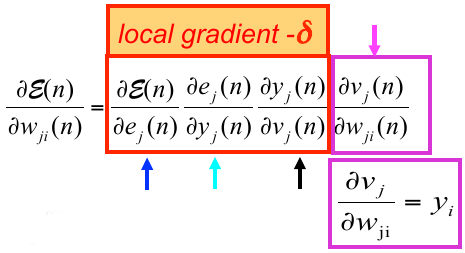
\includegraphics[width=0.9\linewidth]{mlp_bp_breakdown}
        \end{wrapfigure}
        \[ \Rightarrow \Delta w_{ji}(n) = -\eta \delta_j y_i(n) \]

        2 cases:
        \begin{itemize}
            \item $ j $ is an output neuron
            \item $ j $ is a hidden neuron
        \end{itemize}
    \end{alertblock}
    \begin{alertblock}{Local gradient -- output neuron}
        \picEqHereWidth{mlp_bp_localgrad_1}{0.6\linewidth}
        \[ \Rightarrow \delta_j = e_j \phi'(v_j) = (d_j - y_j) \phi'(v_j) \]
    \end{alertblock}
\end{frame}

%-------------------------------------------------
\begin{frame}{Back-propagation for MLP}
    \begin{alertblock}{Local gradient -- hidden neuron}
        Since $ e_j = d_j - y_j $ is missing, reformulate local gradient and apply chain rule:
        \[ \delta_j = \cfrac{\delta \mathbf{\mathcal{E}}}{\delta y_j} \frac{\delta y_j}{\delta v_j} = \phi'(v_j) \sum_{k \in C} \delta_k w_{kj}) \]
        where $ \phi'(v_j) = ay_j(1-y_j) $ (in which $ a > 0 $)
    \end{alertblock}
    \begin{alertblock}{BP algorithm}
        \begin{itemize}
            \item Forward: run NN \& compute error for each neuron of output layer
            \item Backward: pass errors backwards from output layer, by recursively computing local gradient of each neuron.
        \end{itemize}
    \end{alertblock}
    \begin{alertblock}{Stopping criterion}
        \begin{itemize}
            \item absolute rate of change in average squared error small enough
            \item test NN for generalization after each epoch, stop if performance adequate.
        \end{itemize}
    \end{alertblock}
\end{frame}

%-------------------------------------------------
\begin{frame}{Back-propagation for MLP}
    \begin{alertblock}{Generalization}
        Generalize well if the produced mapping works well with new data. May over-fit and memorize the data if NN learns to many examples. Influencing factors:
        \begin{itemize}
            \item size of training set
            \item architecture of NN
            \item complexity of problem
        \end{itemize}
    \end{alertblock}
    \begin{alertblock}{Expressive capability}
        \begin{itemize}
            \item Every \textbf{boolean} function can be represented by NN with \textbf{1 hidden layer}, but may require \textbf{exponential hidden units}
            \item Every \textbf{bounded continuous} can be approximated with arbitrarily small error by NN with \textbf{1 hidden layer}
            \item \textbf{Any function} can be approximated with arbitrary accuracy by NN with \textbf{2 hidden layer}
        \end{itemize}
    \end{alertblock}
\end{frame}

%-------------------------------------------------
\begin{frame}{Back-propagation for MLP}
    \begin{alertblock}{Convergence: Generalized Delta Rule}
        \begin{itemize}
            \item Hard to choose learning rate:\\
                $ \eta $ small $ \rightarrow $ slow rate of learning,\\
                $ \eta $ large $ \rightarrow $ NN can become unstable
            \item Solution: add momentum $ \rightarrow $ generalized delta rule:
                \picEqHereWidth{mlp_generalized_delta}{0.5\linewidth}
            \item Momentem $ \alpha $ (1) accelerates descent in steady downhill directions and (2) stabilizes directions oscillating in time.
        \end{itemize}
    \end{alertblock}
    \begin{alertblock}{$ \eta $ Adaptation}
        \begin{itemize}
            \item Heuristic 1: every weight has own $ \eta $
            \item Heuristic 2: every $ \eta $ can vary from one iteration to the next
        \end{itemize}
    \end{alertblock}
\end{frame}

%-------------------------------------------------
\begin{frame}{Radial Basis Function}
    \begin{alertblock}{Cover's Theorem}
        $ \{ \phi_i(x) \}_{i=1}^{m_1} $: family of $ m_1 $ nonlinear functions
        \begin{itemize}
            \item binary partition $ C^1, C^2 $ of training set $ C $ is \textbf{$ \phi $-separable} if $ \exists w $ of dimension $ m_1 $ s.t.: $ w^T \phi(x) > 0$ $\forall x \in C^1 $, and $ w^T \phi(x) < 0$ $\forall x \in C^2 $
            \item theorem: probability that randomly picked partition $ C^1, C^2 $ of $ C $ is $ \phi $-separable:
            \[ P(N, m_1) = \left(\frac{1}{2}\right)^{N-1}\sum_{m=0}^{m_1-1}\binom{N-1}{m} \]
            for number of data points $ N > m_1 - 1 $
            \item corollary: \textbf{expected maximum} number of \textbf{randomly assigned} patterns that are \textbf{linearly separable} in a feature space of \textbf{dimension} $ \mathbf{m_1} $ is $ \mathbf{2 m_1} $
        \end{itemize}
    \end{alertblock}
    \begin{alertblock}{RBF architechture}
        \begin{itemize}
            \item hidden layer: nonlinear transformation from input space to hidden space
            \item output layer: linear transformation from hidden space to output space
        \end{itemize}
    \end{alertblock}
\end{frame}

%-------------------------------------------------
\begin{frame}{Radial Basis Function}
    \begin{alertblock}{Interpolation problem}
        \begin{itemize}
            \item Problem: given points $ (x_i, t_i) , x_i \in \mathbb{R}^{m_0}, t_i \in \mathbb{R}, 1<i<N $, find $ \mathbf{F}: \mathbb{R}^{m_0} \mapsto \mathbb{R} $ s.t. $ \mathbf{F(x_i)} = t_i $
            \item RBF solution: $ \mathbf{F(x)} = \sum_{i}w_i\phi(||\mathbf{x}-\mathbf{x_i}||) \Rightarrow \mathbf{w} = \mathbf{\Phi^{-1}t} $
            \item Michelli's theorem: if $ \mathbf{x_i} $ are distinct, $ \mathbf{\Phi} $ is non-singular. Valid RBF families:
            \picEqHereWidth{rbf_valid_func}{0.7\linewidth}
        \end{itemize}
    \end{alertblock}
    \begin{alertblock}{RBF with regularization}
        $ \mathbf{w} = (\mathbf{G} + \lambda \mathbf{I})^{-1} \mathbf{t} $, where $ G_{kl} = \mathbf{G(x_k, x_l)} $ and $ G() $ is a Green's function
    \end{alertblock}
\end{frame}

%-------------------------------------------------
\begin{frame}{Radial Basis Function}
    \begin{alertblock}{Generalized RBFN}
        Use only $ K $ radial functions with only centers $ \mathbf{c_i} $ where $ K << $ number of pattern $ P $: $ \mathbf{F(x)} = \sum_{i=1}^{K}w_i\phi(||\mathbf{x}-\mathbf{c_i}||) $
    \end{alertblock}
    \begin{alertblock}{Comparison with MLP}
        \centering
        \begin{tabular}{p{0.3\linewidth} p{0.3\linewidth}p{0.3\linewidth}}
            & RBFN & MLP \\
            \hline
            number of hidden layers & single & single or multiple \\
            linear-ness & nonlinear hidden, linear output & nonlinear hidden, linear/nonlinear output \\
            argument of hidden & Euclidean norm & scalar product \\
            approximation property & universal & universal \\
            approximators scope & local & global \\
            learning & splitted & global
        \end{tabular}
    \end{alertblock}
    \begin{alertblock}{Computation of centers}
        Centers $ \mathbf{c_i} $ must have (density) properties of data points $ \mathbf{x_i} $
    \end{alertblock}
\end{frame}

%-------------------------------------------------
\begin{frame}{Radial Basis Function}
    \begin{alertblock}{k-means}
        \picEqHereWidth{rbfn_kmeans}{\linewidth}
    \end{alertblock}
\end{frame}

%-------------------------------------------------
\begin{frame}{Support Vector Machines}
    \begin{alertblock}{Maximum margin}
        \begin{itemize}
            \item Simplest SVM: linear SVM (LSVM) $ \equiv $ maximum margin linear classifier
            \item Support vectors: data points that margin pushes up against
            \item Margin width: $ M = \cfrac{2}{\sqrt{\mathbf{w} . \mathbf{w}}} $
        \end{itemize}
    \end{alertblock}
    \begin{alertblock}{Learn maximum margin}
        For R data points, minimize (error term for handling noise): $ \frac{1}{2} \mathbf{w} . \mathbf{w} + C \sum_{k=1}^{R}\epsilon_k $ \\
        2R constraints:
        \picEqHereWidth{svm_constraints}{0.3\linewidth}
    \end{alertblock}
    \begin{alertblock}{Nonlinear basis function}
        Common SVM basis functions $ \mathbf{z}_k $: (1) polynomial terms, (2) radial basis functions, or (3) sigmoid of $ \mathbf{x}_k $
    \end{alertblock}
\end{frame}

%-------------------------------------------------
\begin{frame}{Support Vector Machines}
    \begin{alertblock}{Quadratic programming}
        \picEqHereWidth{svm_qp}{\linewidth}
        Can be simplified by observing $ \mathbf{\Phi(a) . \Phi(b)} = (\mathbf{a . b} +1)^2 $
    \end{alertblock}
    \begin{alertblock}{VC dimension}
        \picEqHereWidth{svm_vcdim}{0.4\linewidth}
    \end{alertblock}
\end{frame}

%-------------------------------------------------
\begin{frame}{Self-Organizing Maps}
    \begin{alertblock}{SOM algorithm basics}
        \begin{itemize}
            \item Winner Takes All (WTA) algorithm
            \item 2 layers
            \begin{itemize}
                \item input layer: fully connected to each neuron in 2\textsuperscript{nd} layer
                \item map layer: 1D/2D/3D, organized as line/square/cube
            \end{itemize}
            \item Goal: find weight vectors connecting inputs to each node of lattice s.t.:
            \begin{itemize}
                \item adjacent neurons have similar weight vectors
                \item output of NN will be neuron whose weight vector is most similar to input
                \item each neuron is a \textbf{center of a cluster} containing all inputs mapped to it
            \end{itemize}
            \item Essential ingredients:
            \begin{itemize}
                \item continuous input space of activation patterns generated in accordance with a probability distribution
                \item topology of the network: a lattice of neurons defining discrete output space
                \item time-varying neighborhood function $ h_{ij(x)}(n) $ defined around a winning neuron $ i(x) $
                \item decreasing learning rate parameters $ h(n) $ starting at $ h_0 $ but never goes to $ 0 $
            \end{itemize}
        \end{itemize}
    \end{alertblock}
\end{frame}

%-------------------------------------------------
\begin{frame}{Self-Organizing Maps}
    \begin{alertblock}{Algorithm summary}
        \begin{itemize}
            \item Initialization: choose random, small weight vectors unique for each neuron
            \item Sampling: draw sample $ x $ from input space
            \item Similarity matching: find winning neuron $ i(x) $ at step $ n $
                \[ i(x) = \arg\min_j ||x(n) - w_j|| \]
            \item Updating: adjust weight vectors:
                \picEqHereWidth{som_weight_update}{0.5\linewidth}
            \item Continuation: go to sampling step until no more changes in feature map
        \end{itemize}
    \end{alertblock}
    \begin{alertblock}{Learning characteristics}
        \begin{itemize}
            \item neurons not in neighborhood left unchanged
            \item starts with neighborhood size $ \lambda $ and gradually reduces it
            \item and gradually reduces learning rate $ \eta $
        \end{itemize}
    \end{alertblock}
\end{frame}

%-------------------------------------------------
\begin{frame}{Self-Organizing Maps}
    \begin{alertblock}{Essential processes}
        \begin{enumerate}
            \item Competition: choose best matching neuron, input space mapped to discrete output space
            \item Cooperation:
            \begin{itemize}
                \item winning neuron locates center of neighborhood of cooperating neurons
                \item this neighborhood depends on lateral distance $ d_{ij} $ between winning neuron $ i $ and neuron $ j $
                \item neighborhood function -- Gaussian:
                \picEqHereWidth{som_nbh_gaussion}{0.3\linewidth}
                where $ \sigma $ decays with time \& $ d_{ji} $ is the lateral distance
            \end{itemize}
            \item Weight adaptation:
                \picEqHereWidth{som_weight_update2}{0.6\linewidth}
        \end{enumerate}
    \end{alertblock}
\end{frame}

%-------------------------------------------------
\begin{frame}{Self-Organizing Maps}
    \begin{alertblock}{2 phases of weight adaptation}
        \begin{itemize}
            \item Ordering phase: topological ordering of weight vectors (1k iterations). Parameter choices:
            \begin{itemize}
                \item $ \eta(n) $: $ \eta_0 = 0.1, T_2=1000 $
                \item $ h_{ji(x)}(n) $: $ \sigma_0$ big enough, $T_1=\cfrac{1000}{\log(\sigma_0)} $
            \end{itemize}
            \item Convergence phase: fine tune feature map (10k iterations). Parameter choices:
            \begin{itemize}
                \item $ \eta(n) $ maintained on order of $ 0.01 $
                \item $ h_{ji(x)}(n) $ eventually reduces to 1 or 0 neighboring neurons
            \end{itemize}
        \end{itemize}
    \end{alertblock}
\end{frame}

%-------------------------------------------------
\begin{frame}{Echo State Networks}
    Bifurcation: qualitative change induce by control parameters
    \begin{alertblock}{Backpropagation through time (BPTT)}
        \begin{itemize}
            \item stack network time steps and use backprop like with feedforward network
            \item problems:
            \begin{itemize}
                \item passing through bifurcation: error function does not change smoothly
                \item error gradient information diverges/shrink exponentially
                \item trapped in local optimum
                \item non-local info needed
                \item computationally costly
                \item algorithms are difficult
            \end{itemize}
        \end{itemize}
    \end{alertblock}
\end{frame}

%-------------------------------------------------
%   END
%-------------------------------------------------
\end{document}
